Perceptron, developed by Frank Rosenblatt in 1958 \cite{perceptronprobabmodel}, is the simplest class of artificial neurons.

Perceptron takes several binary inputs in form of a vector $\vec{x} = (x_1, x_2,...,x_n)$, and outputs a single binary number. Perceptron uses real numbers called \textit{weights}, assigned to each edge, vector $\vec{w} = (w_1,w_2,...,w_n)$, to express the importance of respected input edges, 

A \textit{step function} calculates the perceptron's output.
The function output is either 0 or 1 determined by whether its weighted sum $\alpha = \sum_{i} x_i w_i$ is less or greater than its \textit{threshold} value, a real number, usually represented as an incoming edge with a negative weight -1 \cite{matous}.

\begin{equation}
    output =
\begin{cases}
    1, & \text{if $\alpha\ \geq\ threshold$}\\
    0, & \text{if $\alpha\ <\ threshold$}
\end{cases} 
\end{equation} 


\begin{figure}[h]
	\centering
    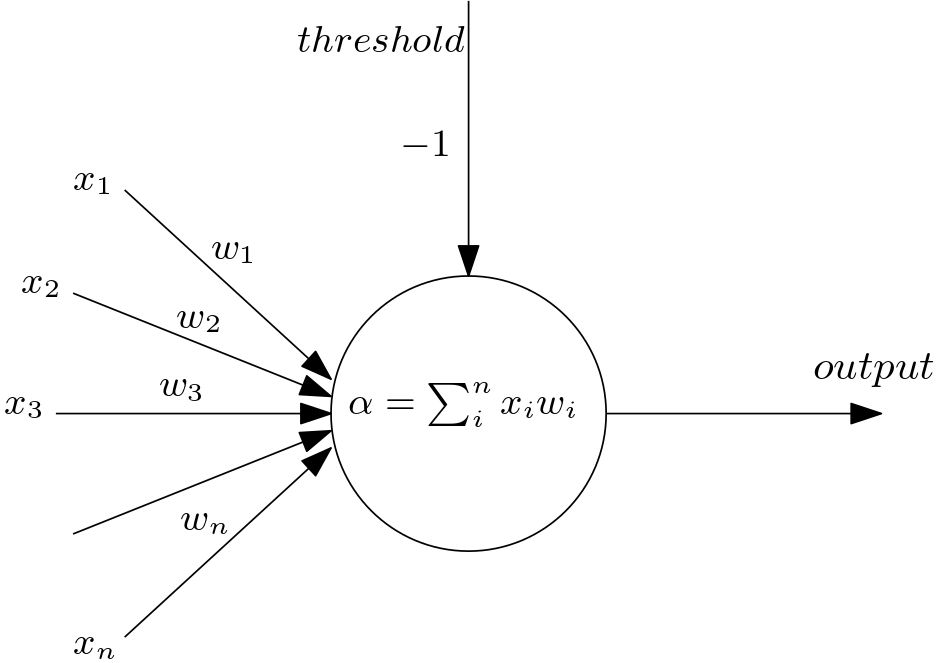
\includegraphics[width=12cm]{perceptron.png}
	\caption{Perceptron \cite{matous}}
	\label{fig:perceptron}
\end{figure}
